\section{}
The free vibration of a viscously damped SDOF system due to a non-zero initial 
displacement (zero initial velocity) is given in the graph shown below. Determine the 
following questions using this graph. Clearly indicate the values you obtain from the graph.

\begin{figure}[h]
\centering
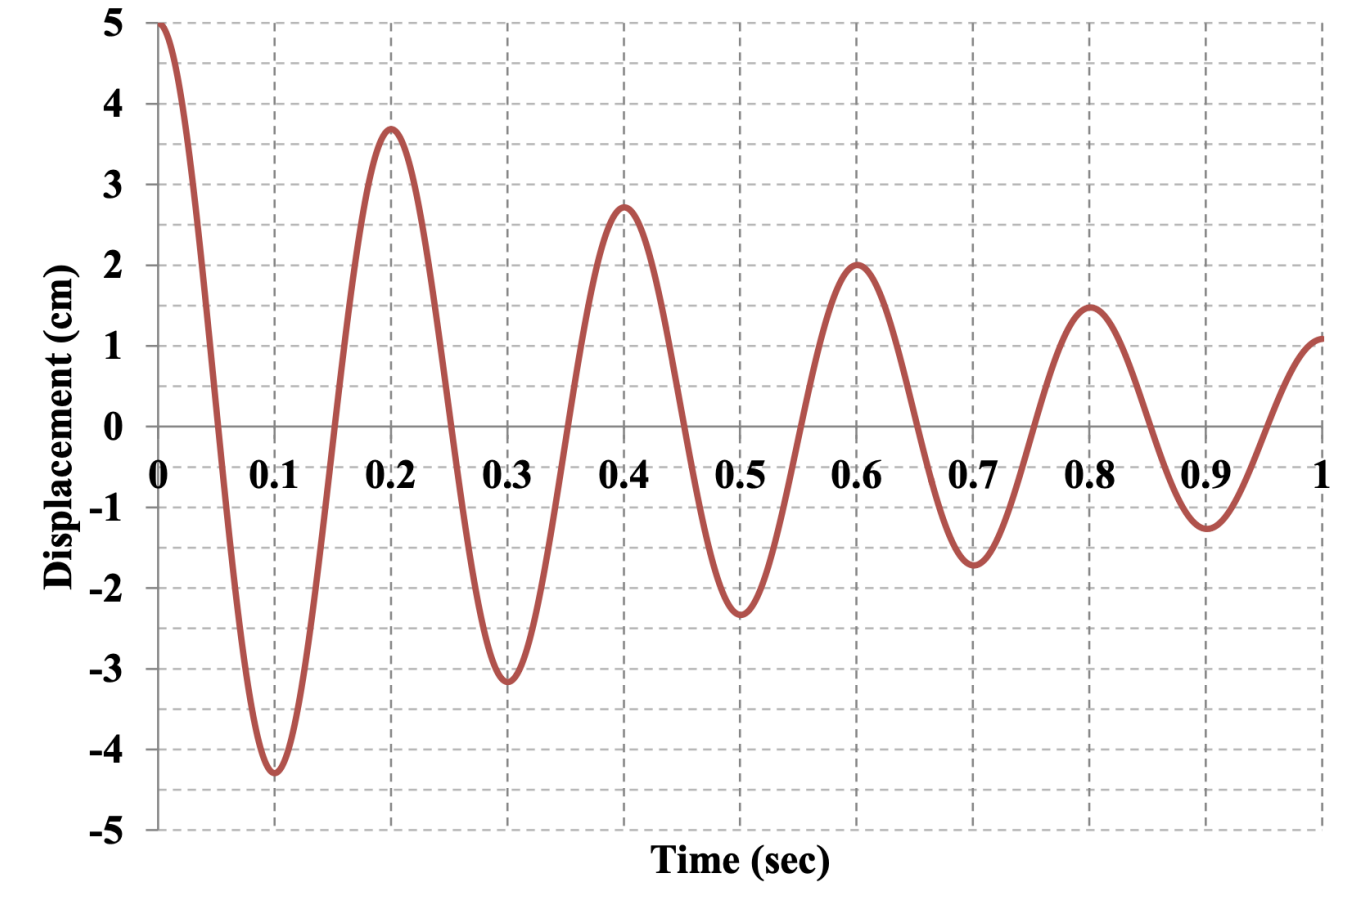
\includegraphics[width=0.5\textwidth]{Questions/Figures/q1 Graph.png}
\end{figure}

\begin{enumerate}[label=(\alph*)]
    \item (5 pts) Write a differential equation that governs the equation of motion of this 
    system.
    \item (5 pts) If the same system was subjected only to a non-zero initial velocity of 
    100cm/sec (zero initial displacement), what would be the displacement response at 
    t = 0.25 sec.
\end{enumerate}

\subsection*{Solution}
\subsection{}

Notice that the graph exhibits the behaviour of a damped cosine wave. Using $x_0= 5$ and $x_3 = 2$, 
\begin{align*}
    \delta &= \frac{1}{n} \ln\left(\frac{x_0}{x_3}\right) \\
    &= \frac{1}{3} \ln\left(\frac{5}{2}\right) \\
    &= 0.30543
\end{align*}
From this, we can find the damping ratio $\zeta$,
\begin{align*}
    \zeta &= \frac{\delta}{\sqrt{4\pi^2 + \delta^2}} \\
    &= \frac{0.30543}{\sqrt{4\pi^2 + 0.30543^2}} \\
    &= 0.048553
\end{align*}
The period is $\tau = 0.1$ sec, so the natural frequency is 
\begin{align*}
    p &= \frac{2\pi}{\sqrt{1-\zeta^2} \tau} \\
    &= \frac{2\pi}{\sqrt{1-0.048553^2} \cdot 0.1} \\
    &= 62.91 \text{ rad/sec}
\end{align*}
Recall the equation of motion for a damped SDOF system,
\begin{align*}
    m\ddot{x} + c\dot{x} + kx = 0
\end{align*}
dividing by $m$ and letting $p^2 = \frac{k}{m}$ and $2\zeta p = \frac{c}{m}$, we get
\begin{align*}
    \ddot{x} + 2\zeta p\dot{x} + p^2x = 0
\end{align*}
substituting in the values we found, we get
\begin{gather*}
    \ddot{x} + 2(0.048553)(62.91)\dot{x} + (62.91)^2x = 0 \\
    \boxed{\ddot{x} + 6.11\dot{x} + 3957.7x = 0}
\end{gather*}

\subsection{}
The general solution to the damped SDOF system is given by
\begin{align*}
    x(t) = e^{-\zeta p t}\left(A\sin\left(\sqrt{1-\zeta^2}pt\right) + B\cos\left(\sqrt{1-\zeta^2}pt\right)\right)
\end{align*}
where $A$ and $B$ are constants. We can find these constants using the initial conditions. The initial displacement can be found from the graph to be 5 cm.
\begin{align*}
    x(0) &= 5 = A 
\end{align*}
Now, using initial velocity of 100 cm/sec, using (3.13) from the course notes, 
\begin{align*}
    x(t) = e^{-\zeta p t}\left(\frac{v_0 + \zeta p x_0}{\sqrt{1-\zeta^2}}\sin\left(\sqrt{1-\zeta^2}pt\right) + x_0\cos\left(\sqrt{1-\zeta^2}pt\right)\right)
\end{align*}
so,
\begin{align*}
    x(0.25) &= e^{-0.048553 \cdot 62.91 \cdot 0.25}\left(\frac{100 + 0.048553 \cdot 62.91 \cdot 5}{\sqrt{1-0.048553^2}}\sin\left(\sqrt{1-0.048553^2}62.91\cdot 0.25\right) \right. \\
    &\quad \left. + 5\cos\left(\sqrt{1-0.048553^2}62.91\cdot 0.25\right)\right) \\
    &= \boxed{-2.383 \text{ cm}}
\end{align*}